\documentclass[a4paper,12pt,oneside]{book}

%-------------------------------Start of the Preable------------------------------------------------
\usepackage[english]{babel}
\usepackage{blindtext}
\usepackage{float}
%packagr for hyperlinks
\usepackage{hyperref}
\hypersetup{
    colorlinks=true,
    linkcolor=blue,
    filecolor=magenta,      
    urlcolor=cyan,
}

\urlstyle{same}
%use of package fancy header
\usepackage{fancyhdr}
\setlength\headheight{26pt}
\fancyhf{}
%\rhead{
\includegraphics[width=1cm]{logo}}
\lhead{\rightmark}
\rhead{
\includegraphics[width=1cm]{logo}}
\fancyfoot[RE, RO]{\thepage}
\fancyfoot[CE, CO]{\href{http://www.e-yantra.org}{www.e-yantra.org}}

\pagestyle{fancy}

%use of package for section title formatting
\usepackage{titlesec}
\titleformat{\chapter}
  {\Large\bfseries} % format
  {}                % label
  {0pt}             % sep
  {\huge}           % before-code
 
%use of package tcolorbox for colorful textbox
\usepackage[most]{tcolorbox}
\tcbset{colback=cyan!5!white,colframe=cyan!75!black,halign title = flush center}

\newtcolorbox{mybox}[1]{colback=cyan!5!white,
colframe=cyan!75!black,fonttitle=\bfseries,
title=\textbf{\Large{#1}}}

%use of package marginnote for notes in margin
\usepackage{marginnote}

%use of packgage watermark for pages
%\usepackage{draftwatermark}
%\SetWatermarkText{
\includegraphics{logo}}
\usepackage[scale=2,opacity=0.1,angle=0]{background}
\backgroundsetup{
contents={
\includegraphics{logo}}
}

%use of newcommand for keywords color
\usepackage{xcolor}
\newcommand{\keyword}[1]{\textcolor{red}{\textbf{#1}}}

%package for inserting pictures
\usepackage{graphicx}

%package for highlighting
\usepackage{color,soul}

%new command for table
\newcommand{\head}[1]{\textnormal{\textbf{#1}}}


%----------------------End of the Preamble---------------------------------------


\begin{document}

%---------------------Title Page------------------------------------------------
\begin{titlepage}
\raggedright
{\Large eYSIP2016\\[1cm]}
{\Huge\scshape Raspberry Pi Hardware Development \& Tutorials \\[.1in]}
\vfill
\begin{flushright}
{\large Aditya Kumar \\}
{\large Pritish Salunke \\}
{\large Rutuja Ekatpure \\}
{\large Deepa Avudiappan \\}
{\large Duration of Internship: $ 21/05/2016-10/07/2016 $ \\}
\end{flushright}

{\itshape 2016, e-Yantra Publication}
\end{titlepage}
%-------------------------------------------------------------------------------

\chapter[Project Tag]{Raspberry Pi Hardware Development \& Tutorials}
\section*{Abstract}
Interfacing LED, switch, LCD and ICs on Raspberry Pi. Create a module of each device interfaced. Communication between Raspberry Pi and other device using Zigbee and Bluetooth module.Communication between Raspberry Pi and Firebird V using SPI, I2C and UART protocol. Create documentation and video tutorial explaining individual module. Design PCB for the devices interfaced with Raspberry Pi.

\subsection*{Completion status}
\begin{itemize}
    \item \textbf{Task 1:}  \\ 
            Learnt, tested and developed different modules for Raspberry Pi \\
            E.g. PWM Driver IC PCA9685, ADC, Port Expander etc. \\
    \item \textbf{Task 2:} \\
            Communication between Rpi and other
            device through Xbee and Bluetooth Module \\
    \item \textbf{Task 3:} \\
            Interfacing LCD with Raspberry Pi  \\
    \item \textbf{Task 4:}  \\
            Communication between Raspberry Pi and 
            Firebird V using UART communication protocol    \\
    \item \textbf{Task 5:}  \\
            Communication between Raspberry Pi  
            and Arduino UNO       
            using I2C and SPI protocol     \\
    \item \textbf{Task 6:} \\
            Designed PCBs for: \\
            \begin{enumerate}
            \item LCD connected with port expander IC MCP23017 IC
            \item LM35 temperature sensor and Sharp IR sensor with ADC IC MCP3008
            \item PWM driver IC PCA9685 to drive DC motor and Servo motor 
            \item Xbee and Bluetooth module 
            \end{enumerate}
    \item \textbf{Task 7:} \\
            Challenge Activity
              
\end{itemize}
    


\section{Hardware parts}
\begin{itemize}
  \item List of hardware 
  \begin{enumerate}
      \item Raspberry Pi \\
      \begin{figure}[H]
        \centering
        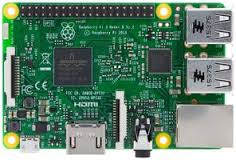
\includegraphics[scale=0.6]{RPi}
        \caption{Raspberry Pi}
      \end{figure}
      \href{https://cdn-shop.adafruit.com/pdfs/raspberrypi2modelb.pdf} {Download link}
      \href{http://www.amazon.in/Raspberry-Pi-Model-1GB-Complete/dp/B00T2U7R7I} {Vendor Link}
      \item FireBird V Robot \\
      \begin{figure}[H]
        \centering
        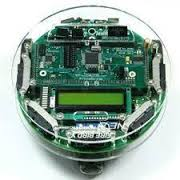
\includegraphics[scale=0.6]{Firebird_V_robot}
        \caption{Firebird V robot}
      \end{figure}
      \href{http://www.atmel.com/Images/Atmel-2549-8-bit-AVR-Microcontroller-ATmega640-1280-1281-2560-2561_datasheet.pdf} {Download link}
      \href{http://www.nex-robotics.com/products/fire-bird-v-robots/fire-bird-v-atmega2560-robotic-research-platform.html} {Vendor Link}
      \item LED
      \item Resistor
      \item Switch
      \item LCD   \\
      \begin{figure}[H]
        \centering
        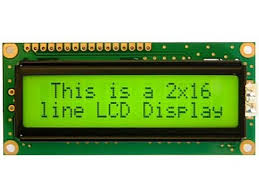
\includegraphics[scale=0.6]{LCD}
        \caption{LCD}
      \end{figure}
      \href{http://www.agspecinfo.com/pdfs/J/JHD162A.PDF} {Download link}
      \href{http://www.amazon.in/JCE-16x2-LCD-Display/dp/B00OVY28M4} {Vendor Link}
      \newpage
      \item MCP23017 IC     \\
      \begin{figure}[H]
        \centering
        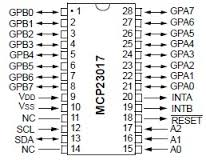
\includegraphics[scale=0.6]{MCp23017}
        \caption{MCP23017 Port Expander IC}
      \end{figure}
      \href{https://cdn-shop.adafruit.com/datasheets/mcp23017.pdf} {Download link}
      \href{http://www.smddevices.com/} {Vendor Link}
      \item MCP3008 IC       \\
      \begin{figure}[H]
        \centering
        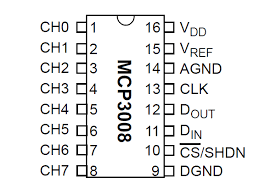
\includegraphics[scale=0.6]{Mcp3008}
        \caption{ADC MCP3008 IC}
      \end{figure}
      \href{https://cdn-shop.adafruit.com/datasheets/MCP3008.pdf} {Download link}
      \href{http://www.dnatechindia.com/MCP3008-10-Bit-ADC.html} {Vendor Link}
      \item Sharp Sensor      \\
      \begin{figure}[H]
        \centering
        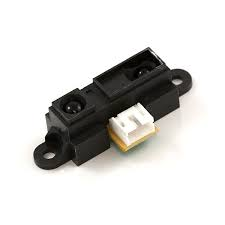
\includegraphics[scale=0.6]{sharp}
        \caption{Sharp IR Sensor}
      \end{figure}
      \href{http://www.sharpsma.com/webfm_send/1208} {Download link}
      \href{http: //www.ebay.in/itm/262401450416?aff_source=Sok-Goog} {Vendor Link}
      \item LM35 Temperature Sensor    \\
      \begin{figure}[H]
        \centering
        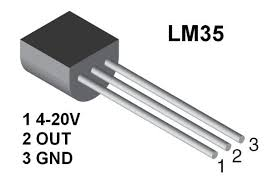
\includegraphics[scale=0.6]{lm35}
        \caption{LM35 Temperature sensor}
      \end{figure}
      \href{http://www.ti.com/lit/ds/symlink/lm35.pdf} {Download link}
      \href{http://www.amazon.in/Robo-India-Temperature-Sensor-LM35/dp/B00WO5AFPE} {Vendor Link}
      \item PCA9685 PWM Driver IC  \\
      \begin{figure}[H]
        \centering
        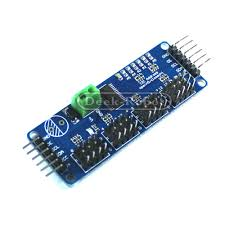
\includegraphics[scale=0.6]{PCA9685}
        \caption{PCA9685 PWM Driver IC}
      \end{figure}
      \href{https://cdn-shop.adafruit.com/datasheets/PCA9685.pdf} {Download link}
      \href{http://www.amazon.in/Channel-Servo-Motor-Driver-Controller-PCA9685/dp/B01D4I8KII?tag=googinhydr18418-21&tag=googinkenshoo-21&ascsubtag=a4459339-54b9-4883-ac3e-2de2611b95a1} {Vendor Link}
      \item L293D Motor Driver IC       \\
      \begin{figure}[H]
        \centering
        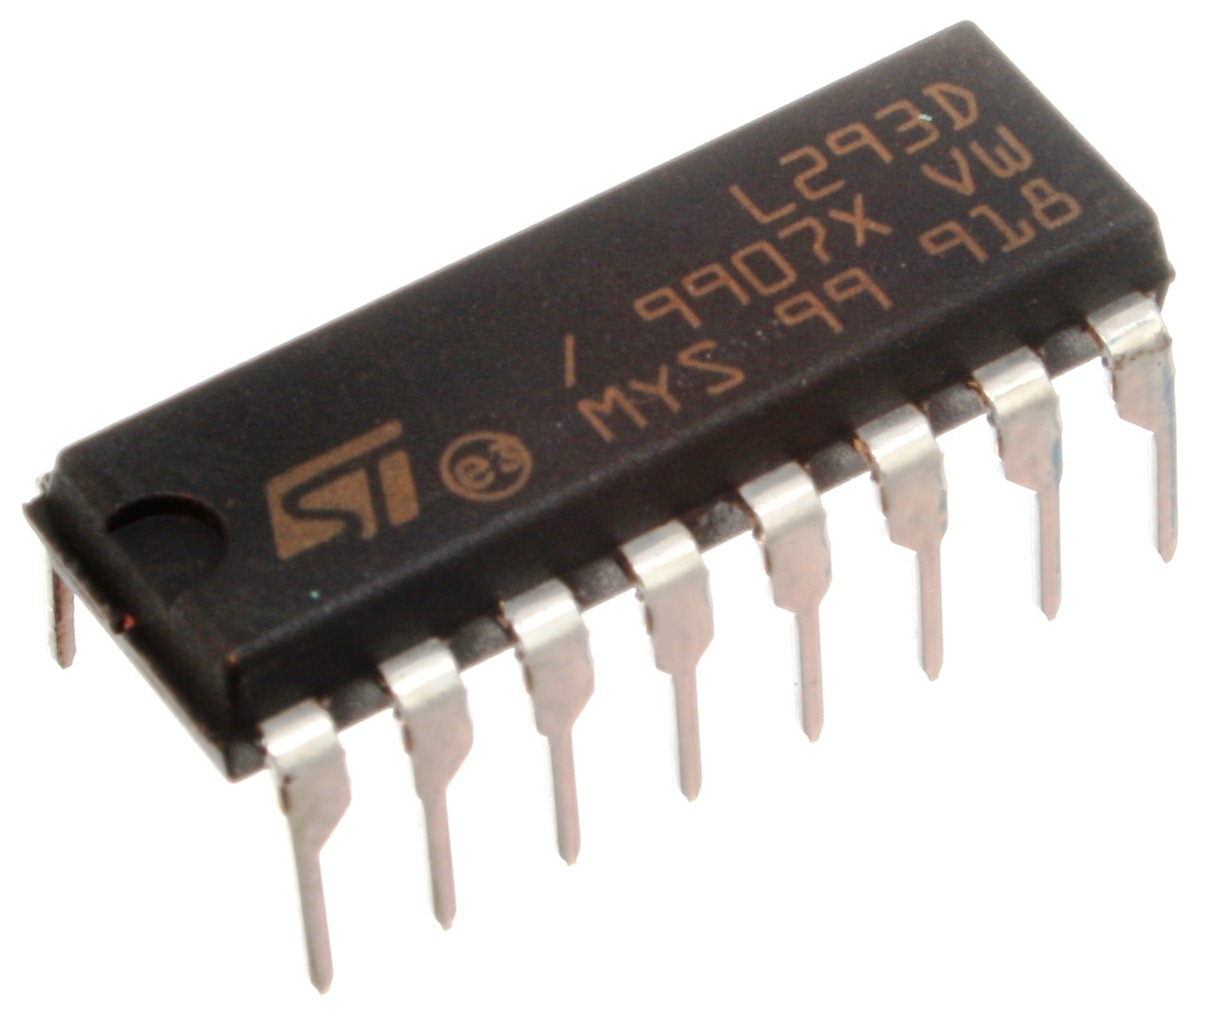
\includegraphics[scale=0.4]{L293D}
        \caption{L293d motor Driver IC}
      \end{figure}
      \href{http://www.ti.com/lit/ds/symlink/l293.pdf} {Download link}
      \href{http://www.amazon.in/L293D-Push-Pull-Four-Channel-Stepper-Driver/dp/B00MYZPL4Y?tag=googinhydr18418-21&tag=googinkenshoo-21&ascsubtag=a4459339-54b9-4883-ac3e-2de2611b95a1} {Vendor Link}
      \item Capacitor
      \item DC Motor
      \begin{figure}[H]
        \centering
        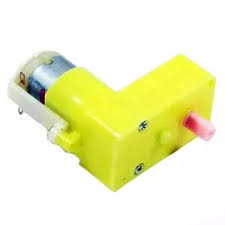
\includegraphics[scale=0.6]{dc}
        \caption{DC motor}
      \end{figure}
      \item Servo Motor
      \begin{figure}[H]
        \centering
        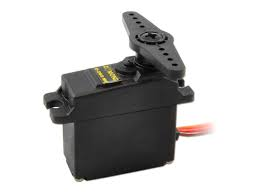
\includegraphics[scale=0.6]{servo}
        \caption{Servo motor}
      \end{figure}
      \item 9 V battery
      \item Xbee Module  \\
      \begin{figure}[H]
        \centering
        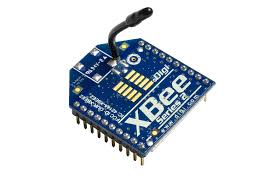
\includegraphics[scale=0.6]{Xbee-1}
        \caption{Xbee}
      \end{figure}
      \begin{figure}[H]
        \centering
        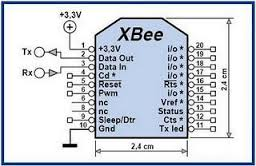
\includegraphics[scale=0.6]{Xbee}
        \caption{Xbee pin diagram}
      \end{figure}
      \href{https://www.sparkfun.com/datasheets/Wireless/Zigbee/XBee-Datasheet.pdf} {Download link}
      \href{http://www.amazon.in/XBee-2mW-Wire-Antenna-ZigBee/dp/B007R9U1QA?tag=googinhydr18418-21&tag=googinkenshoo-21&ascsubtag=a4459339-54b9-4883-ac3e-2de2611b95a1} {Vendor Link}
      \item Bluetooth Module      \\
      \begin{figure}[H]
        \centering
        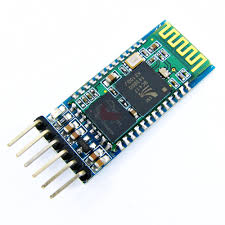
\includegraphics[scale=0.6]{blue}
        \caption{Bluetooth HC-05}
      \end{figure}
      \href{http://www.linotux.ch/arduino/HC-0305_serial_module_AT_commamd_set_201104_revised.pdf} {Download link}
      \href{http://www.amazon.in/Verve-VTA009-Bluetooth-Module-HC-05/dp/B00S15XTG8?tag=googinhydr18418-21&tag=googinkenshoo-21&ascsubtag=a4459339-54b9-4883-ac3e-2de2611b95a1} {Vendor Link}
      \item Arduino UNO   \\
      \begin{figure}[H]
        \centering
        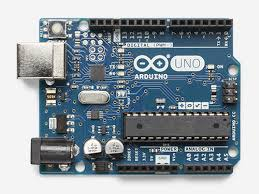
\includegraphics[scale=0.6]{uno}
        \caption{Arduino UNO}
      \end{figure}
      \href{http://www.mouser.com/pdfdocs/Gravitech_ATMEGA328_datasheet.pdf} {Download link}
      \href{http://www.amazon.in/Arduino-UNO-board-DIP-ATmega328P/dp/B008GRTSV6} {Vendor Link}
  \end{enumerate}
\end{itemize}

\section{Software used}
\begin{itemize}
  \item List of software used 
  \begin{enumerate}
      \item MobaXterm Personal Edition \\
      \href{http://mobaxterm.mobatek.net/MobaXterm_Setup_9.1.msi} {Download link}
      \item Raspbian Jessie   \\
      \href{https://downloads.raspberrypi.org/raspbian_latest}{Download Link}
      \item Atmel Studio 6.0 \\
      \href{http://atmel-studio.software.informer.com/download/?ca56297}{Download Link}
      \item Eagle Version 7.6.0 \\
      \href{http://www.cadsoftusa.com/download-eagle/}{Download Link}
      \item NEX ISP USB STK500V2 Programmer \\
      \href{http://www.nex-robotics.com/images/downloads/NEX\%20AVR\%20STK500V2.zip}{Download Link}
      \item XCTU \\
      \href{http://www.digi.com/products/xbee-rf-solutions/xctu-software/xctu#productsupport-utilities}{Download Link}
      \item Arduino 1.6.9  \\
       \href{https://www.arduino.cc/en/Main/Software}{Download Link}
      
      
  \end{enumerate}
\end{itemize}

\section{Accessing GPIO pins of Raspberry Pi}
\flushleft
\textbf{Description:} \\
The Raspberry Pi 1 Model B+ board contains a single 40-pin expansion header providing access to 26 GPIO(General Purpose Input Output) pins. Remaining 14 pins are 3.3V, 5V, Ground.Out of the 26 GPIO pins there are some pins having special functions such as SPI, I2C and UART communication. \\
In order to refer to the R-Pi pins there exists two modes:\\
\begin{enumerate}
    \item BCM mode: Referring the pins with the GPIO number.
    \item Board mode: Referring the pins using the IC pin number.
\end{enumerate}
\textbf{Problem Statement:} \\
LED and switch are connected to different GPIO pins.LED should get ON when switch is pressed once and should get OFF when switch is pressed again.\\
\textbf{Circuit Diagram}\\
\begin{figure}[H]
    \centering
    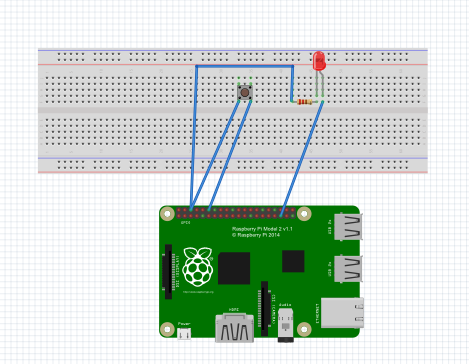
\includegraphics[scale=0.6]{GPIO}
    \caption{}
\end{figure}
\subsection*{Assembly of hardware}
\subsection*{Step 1}
One pin of the push button is connected to Ground(Pin 9).
\subsection*{Step 2}
The other pin of the push button is connected to IC pin no. 12.
\subsection*{Step 3}
The anode of led is connected to IC pin 35 of raspberry pi.
\subsection*{Step 4}
The cathode of led is connected to the the resistor of 300 ohms which
is then connected to the ground.

\section{Enabling I2C interface in Raspberry Pi}
\textbf{Description:} \\
I2C stands for Inter Integrated Circuit. It is a communication protocol in which many devices are connected with two signal line Serial Data(SDA) and Serial Clock(SCL).
Since I2C interface is disabled by default. So, in following steps we have explained how to enable I2C interface on RPi. 
\textbf{Steps to enable I2C interface on RPi}
\begin{enumerate}
		\item Open MobaXterm. 
		\item Establish SSH connection to R-Pi.
		\item  Type \textit{sudo raspi-config}. This will launch the raspi-config utility.
		
		\begin{figure}[H]
			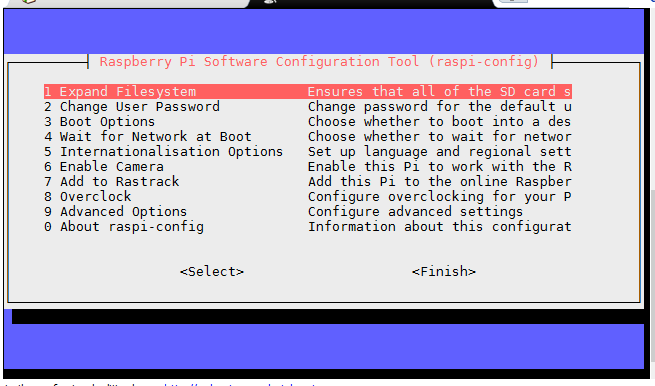
\includegraphics[width=11cm,height=5cm]{i2c_1}
			\centering
			\caption{[4]}
			\end{figure}
		\item Select the \textit{Advanced options}
		\begin{figure}[H]
			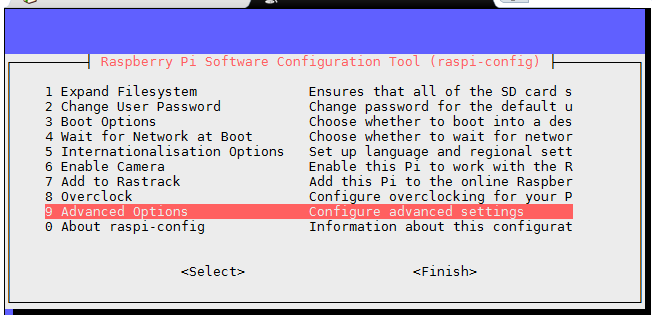
\includegraphics[scale=0.6]{i2c_2}
			\centering
			\caption{[4]}
		\end{figure} 
		\newpage
		\item Then select \textit{option A7 I2C} 
		\newline
		\begin{figure}[h!]
			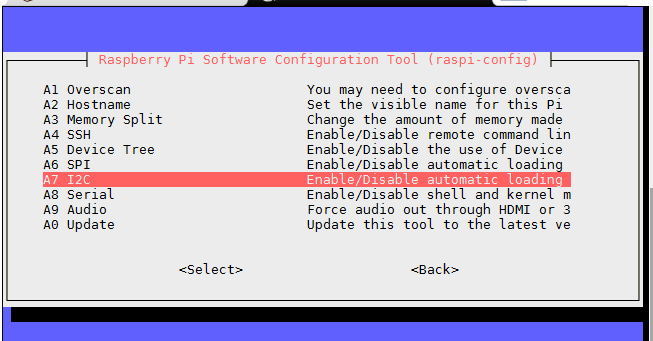
\includegraphics[scale=0.6]{i2c_3}
			\centering
			\caption{[4]}
		\end{figure}
		\item It will ask to enable the ARM I2C interface, click \textit{YES}.
		\newline
		\begin{figure}[h!]
			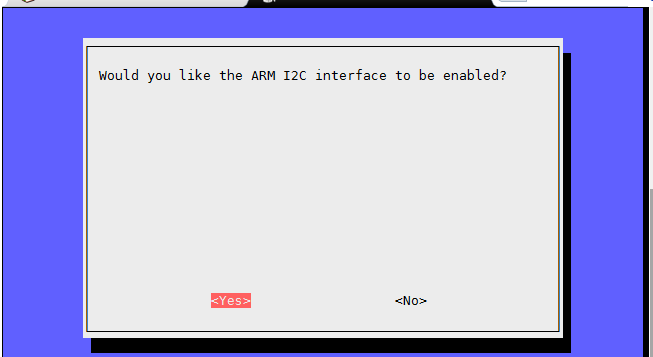
\includegraphics[scale=0.6]{i2c_4}
			\centering
			\caption{[4]}
		\end{figure}
		\newpage
		\item Then it will ask if you would like I2C kernel module to be uploaded by default. Select\textit{YES}.
		\begin{figure}[h!]
			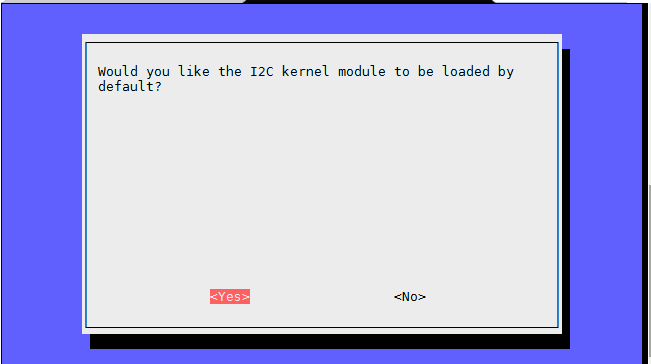
\includegraphics[scale=0.6]{i2c_5}
			\centering
			\caption{[4]}
		\end{figure}
		\item I2C kernel module will now be loaded by default.Click \textit{OK}
		\begin{figure}[h!]
			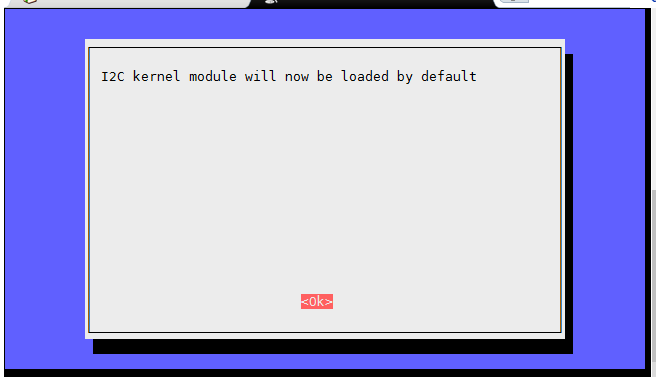
\includegraphics[scale=0.6]{i2c_6}
			\centering
			\caption{[4]}
		\end{figure}
		\item Select Finish to return to command line.
		\item Next we need to edit the modules file using : \newline \textit{sudo nano /etc/modules} 
		\begin{figure}[h!]
			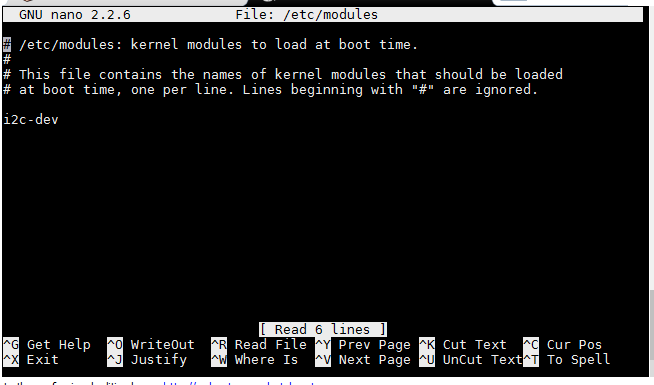
\includegraphics[scale=0.6]{i2c_7}
			\centering
			\caption{[4]}
		\end{figure}
		\newpage
		\item Add the following two lines : \newline \textit{i2c-bcm2708 \newline i2c-dev}
		
		\begin{figure}[h!]
			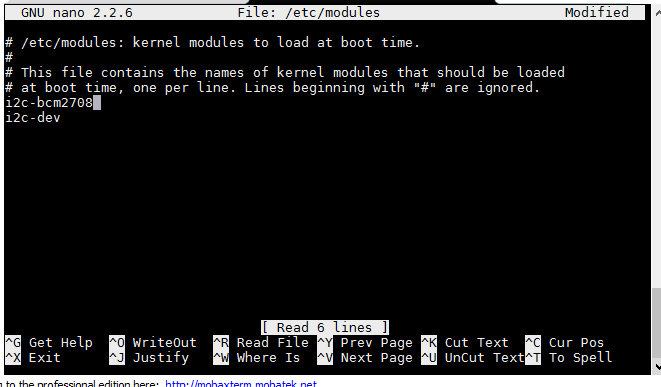
\includegraphics[scale=0.6]{i2c_8}
			\centering
			\caption{[4]}
		\end{figure}
		\item Use CTRL-X, then Y, then RETURN to save the file and exit.
		\item To help debugging and allow the i2c interface to be used within Python we can install “python-smbus” and “i2c-tools” : \newline \textit{sudo apt-get update \newline sudo apt-get install -y python-smbus i2c-tools}
		\item Shutdown your Pi using : \newline \textit{sudo halt} \newline Wait ten seconds, disconnect the power to your Pi and you are now ready to connect your I2C hardware.
		\item When you power up or reboot your Pi you can check the i2c module is running by using the following command : \newline \textit{lsmod | grep i2c\_} \newline That will list all the modules starting with “i2c\_”. If it lists “i2c\_bcm2708” then the module is running correctly.
		\item Once you have connected your hardware double check the wiring. Make sure 3.3V is going to the correct pins and you have got not short circuits. Power up the Pi and wait for it to boot.
		\item Type the command: \newline \textit{sudo i2cdetect -y 1} 
		\item You should the output as:
			\begin{figure}[h!]
				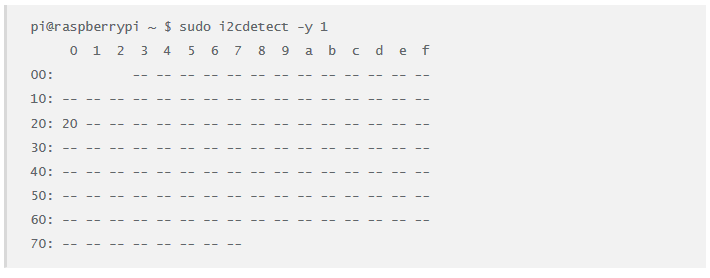
\includegraphics[scale=0.6]{i2c_9}
				\centering
				\caption{[4]}
			\end{figure}	
	\end{enumerate}
\newpage

\section{Interfacing Port Expander MCP23017 IC}
\textbf{Description:}\\
There are only 26 GPIO pins on Raspberry Pi, so when we want to connect more number of actuators, LCD and other peripherals then these pins may be insufficient. So, in order to increase the number of GPIO pins a port expander IC MCP23017 is used. It communicates with Raspberry Pi through I2C protocol. It is a 28 pin IC, providing 16 additional GPIO pins.  \\
\textbf{Problem Statement:} \\
Interfacing LCD to RPi using MCP23017 IC and display some message.\\
\textbf{Circuit Diagram}\\
\begin{figure}[H]
    \centering
    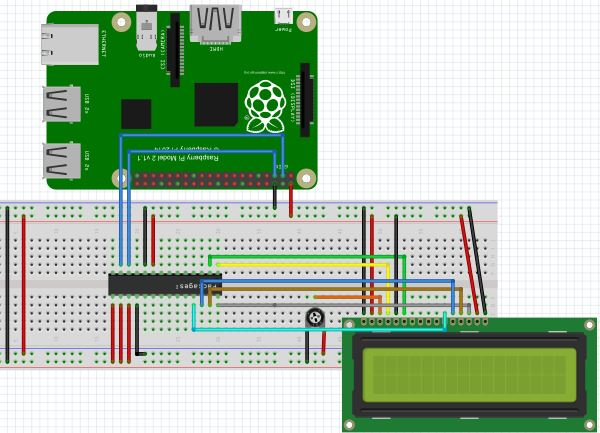
\includegraphics[scale=0.4]{port_expander_lcd}
    \caption{LCD connected to MCP23017 IC}
\end{figure}
\newpage
\textbf{Schematic Diagram}\\
\begin{figure}[H]
    \centering
    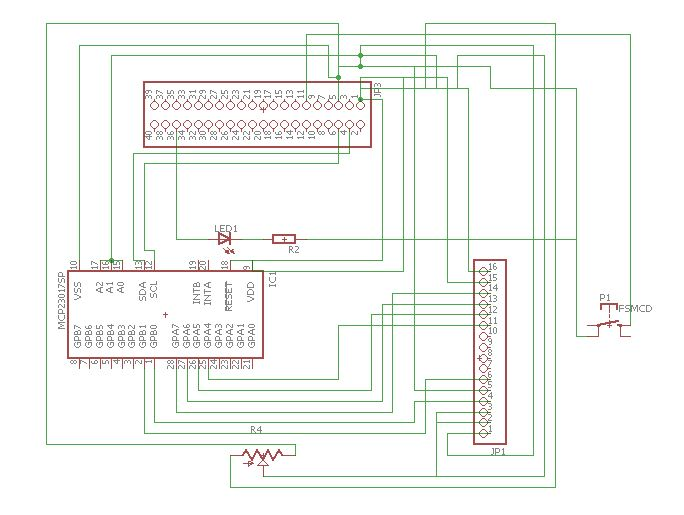
\includegraphics[scale= 0.8]{LCD_schematic}
    \caption{Eagle Schematic}
\end{figure}
\textbf{PCB Layout}\\
\begin{figure}[H]
    \centering
    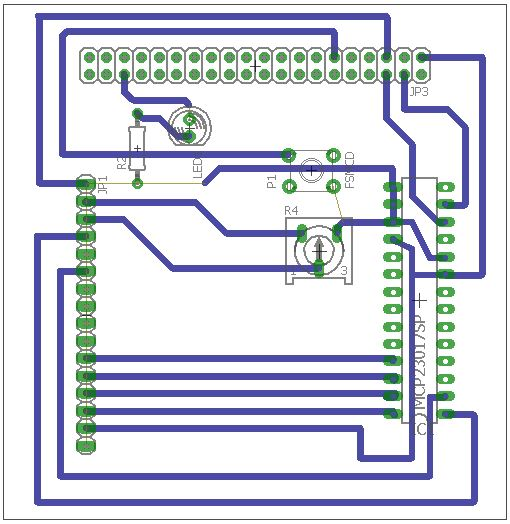
\includegraphics[scale= 0.4]{lcd_pcb_layout}
    \caption{PCB Layout}
\end{figure}
\subsection*{Assembly of hardware}
\subsection*{Step 1}
Pin 9 (VDD) is connected to 5V
\subsection*{Step 2}
Pin 10 (VSS) is connected to Ground
\subsection*{Step 3}
Pin 12 (SCL) is connected to Pin 5 on the Pi GPIO
\subsection*{Step 4}
Pin 13 (SDA) is connected to Pin 3 on the Pi GPIO
\subsection*{Step 5}
Pin 18 (Reset) should be set high for normal operation so we connect this to 5V
\subsection*{Step 6}
Pins 15, 16 \& 17 (A0-A2) determine the number assigned to this device. We are only using one device so we will give it a binary zero by setting all three of these pins to 0 (ground)
\subsection*{Step 7}
RS and Enable pins of the LCD are connected to GPB0 and GPB1 respectively.
\subsection*{Step 8}
R/W pin is Grounded
\subsection*{Step 9}
Data pins D7,D6,D5 and D4 are connected to GPA7,GPA6,GPA5 and GPA4 respectively.

\section{Interfacing ADC IC MCP3008}
\textbf{Description:} \\
Raspberry Pi does not have internal ADC. So, to read the values of analog sensors 
we need to provide external ADC. Here, we will be using MCP3008 IC. 
The MCP3008 is a successive approximation 10bit 8-channel Analogue-to-digital 
converter (ADC). It is cheap, easy to connect and does not require any additional components. It uses the SPI bus protocol which is supported by the Pi's GPIO header.\\
\textbf{Problem Statement:} \\
Read the values of LM35 temperature sensor by using MCP3008 IC(ADC) and calibrate it by programming in python.  \\
\textbf{Circuit Diagram}\\
\begin{figure}[H]
    \centering
    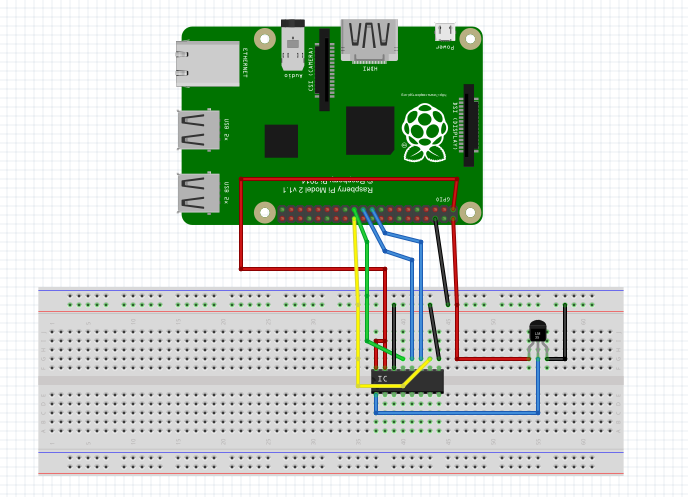
\includegraphics[scale=0.4]{lm35_interfacing}
    \caption{Circuit Diagram}
\end{figure}

\textbf{Schematic Diagram}\\
\begin{figure}[H]
    \centering
    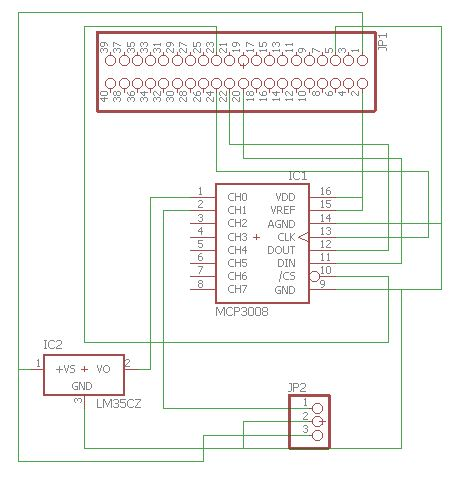
\includegraphics[scale=0.4]{adc_schematic}
    \caption{Schematic in Eagle}
\end{figure}
\textbf{PCB Layout}\\
\begin{figure}[H]
    \centering
    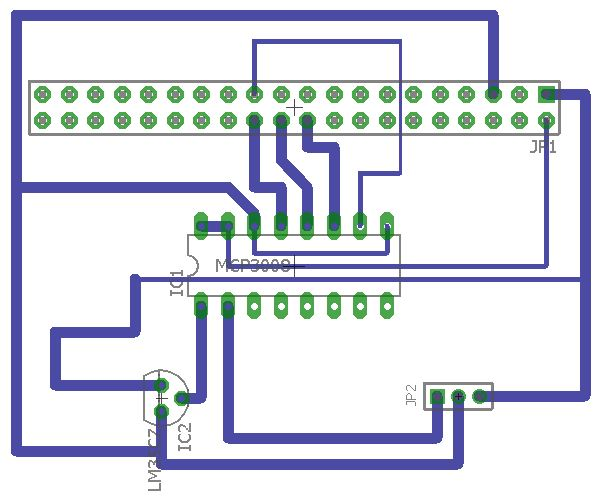
\includegraphics[scale=0.4]{adc_layout}
    \caption{PCB Layout in Eagle}
\end{figure}

\section{Interfacing DC Motor to RPi using MCP23017(Port Expander) IC}
\textbf{Description:} \\
Normal DC gear-head motors require current greater than 250mA. Most of
the ICs like 555 timer,74 series ICs cannot supply this amount of
current.Instead if we directly connect motors to the output of any of the
above IC's, they might get damaged. There is a need of a circuitry that
can act as a bridge between the above mentioned ICs and the motors. This
is where a motor driver plays a crucial role. It regulates the current owing through the circuit hence preventing any damage to the device.
L293D is dual H-bridge motor driver ICs. Using these we can control the
rotation of two motors in both clockwise and anti-clockwise direction. \\
\textbf{Problem Statement:} \\
Controlling the speed of DC motor by using Port expander IC MCP23017 and motor
driver IC L293D. \\
\newpage
\textbf{Circuit Diagram:}\\
\begin{figure}[H]
    \centering
    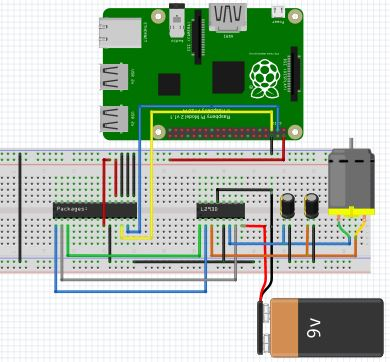
\includegraphics[scale=0.6]{dc_motor_I2C}
    \caption{Fritzing Circuit Diagram}
\end{figure}
\subsection*{Assembly of hardware}
\subsection*{Step 1}
Pin 9 (VDD) is connected to 5V
\subsection*{Step 2}
Pin 10 (VSS) is connected to Ground
\subsection*{Step 3}
Pin 12 (SCL) is connected to Pin 5 on the Pi GPIO
\subsection*{Step 4}
Pin 13 (SDA) is connected to Pin 3 on the Pi GPIO
\subsection*{Step 5}
Pin 18 (Reset) should be set high for normal operation so we connect
this to 5V
\subsection*{Step 6}
Pins 15, 16 \& 17 (A0-A2) determine the number assigned to this device. We are only using one device so we will give it a binary zero by setting all three of these pins to 0 (ground)
\subsection*{Step 7}
Input 1 and Input 2 of L293D is connected to GPB0 and GPB1 of MCP23017
\subsection*{Step 8}
Pin 1 (enable pin) of L293D is connected to GPB2.
\subsection*{Step 9}
Out 1 and Out 2 are connected to a DC motor.

\section{Interfacing Servo motor to RPi using PWM Driver IC PCA9685}
\textbf{Description:} \\
Raspberry Pi has only one pin for PWM generation, which is pin number 12. So, if 
we want to control the speed of more than one motor by changing its PWM then we 
need PCA9685 motor driver IC.
PCA9685 is an I2C-bus controlled 16-channel PWM Driver IC.Each PWM channel output 
has its own 12-bit resolution (4096 steps) fixed frequency individual PWM 
controller that operates at a programmable frequency from a typical of 24 Hz 
to 1526 Hz with a duty cycle that is adjustable from 0% to 100% to allow the motor
to be set to a specific PWM value. All outputs are set to the same PWM frequency.\\
\textbf{Problem Statement:} \\
Controlling the angle or duty ratio of servo motor using PCA9685 PWM Driver IC.
\newpage
\textbf{Circuit Diagram}\\
\begin{figure}[H]
    \centering
    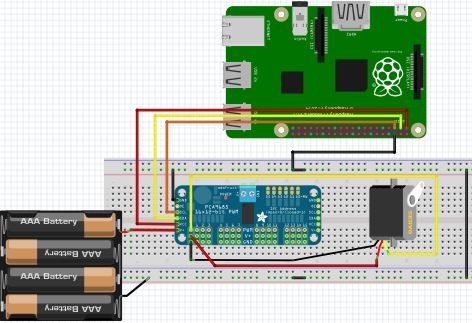
\includegraphics[scale=0.6]{servo_motor_PCA9685}
    \caption{Fritzing Circuit Diagram}
\end{figure}
Fig. above shows connections.
\subsection*{Assembly of hardware}
\subsection*{Step 1}
Control pin of servo motor is connected to S pin of channel 0.
\subsection*{Step 2}
Ground and Vcc of servo motor is connected to ground and Vcc of channel 0 of PCA9685 respectively. 
\subsection*{Step 3}
Pin 12 (SCL) is connected to Pin 5 on the RPi GPIO
\subsection*{Step 4}
Pin 13 (SDA) is connected to Pin 3 on the RPi GPIO
\subsection*{Step 5}
Vcc of IC is connected to pin 2 on the RPi.
\subsection*{Step 6}
Ground pin of IC is connected to pin 6 of RPi.
\subsection*{Step 7}
V+ of IC is connected positive terminal of 9V battery.

\section{Serial Communication using Xbee and Bluetooth Module}
\textbf{Description:} \\
The universal asynchronous receiver/transmitter (UART) takes bytes of data and transmits the individual bits in a sequential fashion. At the destination, a second UART re-assembles the bits into complete bytes. Each UART contains a shift register, which is the fundamental method of conversion between serial and parallel forms.Serial communication is the process of sending data one bit at a time, sequentially, over a communication channel.Asynchronous serial data communication is widely used for character-oriented transmissions.\\
In the asynchronous method, each character is placed
between start and stop bits. This is called framing. In data framing for asynchronous communications, the data, such as ASCII characters, are packed between a start bit and a stop bit. The start bit is always one bit, but the
stop bit can be one or two bits. The start bit is always a 0 (low) and the
stop bit(s) is 1 (high).
\subsection{Bluetooth Module HC-05:}
\textbf{Description:} \\
HC-05 module is an easy to use Bluetooth SPP (Serial Port Protocol) mod-
ule, designed for transparent wireless serial connection setup. It comes with a factory set Baud rate of 9600bps. It is used for serial communication for small distances of few meters. \\
\textbf{Problem Statement:} \\
Establish communication between Raspberry Pi and any other bluetooth enabled device(we have used android device) using Bluetooth module.Check it by sending and receiving data.
\begin{figure}[H]
    \centering
    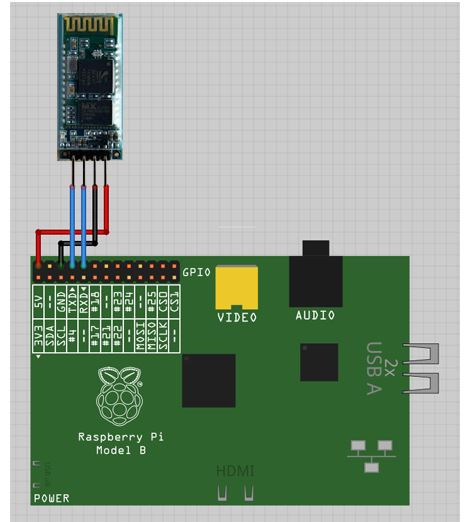
\includegraphics[scale= 0.4]{bluetooth}
    \caption{Connection of Bluetooth module with RPi}
\end{figure}
\subsection*{Assembly of hardware:}
\subsection*{Step 1}
Pin 2 of RPi is connected to Vcc.
\subsection*{Step 2}
Pin 6 of Rpi is connected to ground.
\subsection*{Step 3}
Pin 8(TXD) of RPi is connected to RXD pin.
\subsection*{Step 4}
Pin 10 (RXD) is connected to TXD pin of bluetooth module.
\subsection{Xbee Module:}
\textbf{Description:} \\
Xbee can be used for wireless communication with low power consumption. A 3.6V 600mA Lithium battery may last 6 - 12 months for powering up an Xbee while the wireless range can up to 1 mile. It talks with well known UART interface and makes it easy to use. It is simple and straight forward if you only use 2 Xbee for communication. Xbee is the module using Zigbee protocol. Zigbee is a wireless communication protocol like wifi and bluetooth. \\
\textbf{Problem Statement:} \\
Connect one Xbee to RPi and connect second Xbee to PC(access this module using XCTU software).Check the communication by sending and receiving data serially.
\begin{figure}[H]
    \centering
    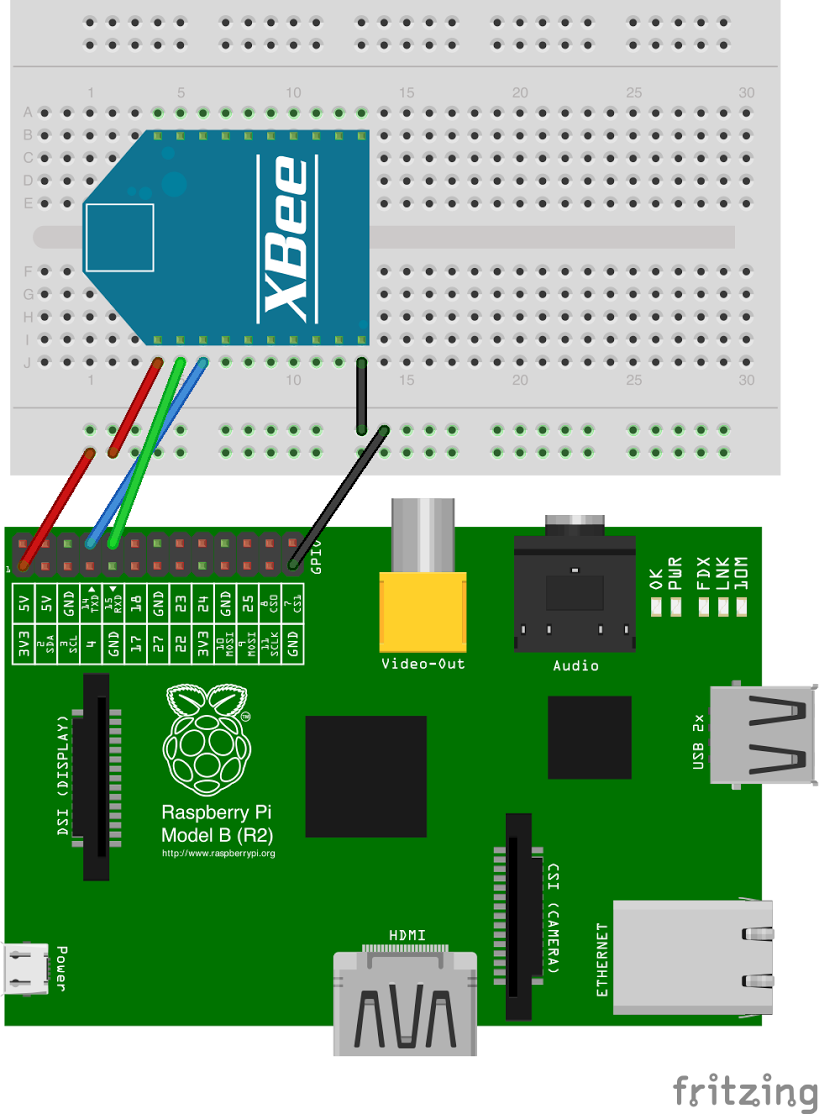
\includegraphics[scale=0.2]{raspi_to_xbee}
    \caption{Connection of Xbee module with RPi}
\end{figure}
\subsection*{Assembly of harware:}
\subsection*{Step 1}
Connect Vcc to pin 2 (5V) of Rpi.
\subsection*{Step 2}
Ground is connected to pin 6 (GND) of RPi.
\subsection*{Step 3}
Pin TXD of Xbee is connected to pin 10 (RXD) of RPi.
\subsection*{Step 4}
Pin RXD of Xbee is connected to pin 8 (TXD) of RPi.
\subsection*{Step 5}
Connect second Xbee to PC through USB cable.\\ 

\textbf{Schematic Diagram of Bluetooth and Xbee Module:}\\
\begin{figure}[H]
    \centering
    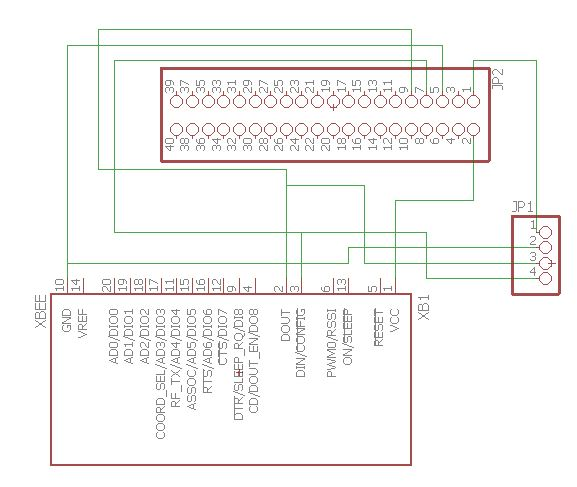
\includegraphics[scale= 0.8]{zigbee_schematic}
    \caption{Schematic in Eagle}
\end{figure}
\newpage
\textbf{PCB Layout}\\
\begin{figure}[H]
    \centering
    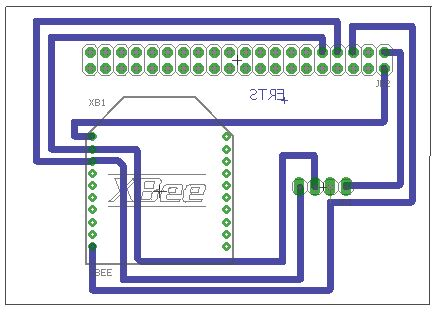
\includegraphics[scale= 0.5]{zigbee_layout}
    \caption{PCB Layout}
\end{figure}

\section{Interrupt on Raspberry Pi}
An Interrupt is a signal generated by some event external to CPU, which causes the CPU to stop what it is doing and go to separate piece of code known as ISR for execution. When the execution of ISR completes it starts main program from where it left.
Types of interrupts are as follows:
\begin{enumerate}
    \item Hardware Interrupt: \\
    Hardware interrupts are used by devices to communicate that they require attention from the operating system.These interrputs are requested by external peripherals such as keyboard, moving the moving trigger.
    \item Software Interrupt: \\
    A software interrupt is a type of interrupt that is caused either by a special instruction in the instruction set or by an exceptional condition in the processor itself. A software interrupt is invoked by software, unlike a hardware interrupt, and is considered one of the ways to communicate with the kernel or to invoke system calls, especially during error or exception handling.
\end{enumerate}
In Raspberry Pi we actually use the concept of multithreading. By multithreading multiple programs can be executed in different threads i.e., multiple tasks can be executed at the same time.\\
\newpage
\subsection*{External Interrupt on RPi:}
\textbf{Description:} \\
Interrupt can be generated externally on Raspberry Pi by logic devices such as switch or push button which changes the logic when they are pressed. \\
\textbf{Problem Statement:} \\
Connect a switch to any one of the GPIO pin and connect two LED's to the two other GPIO pins.One LED should blink continously with a time delay of 1 second and other LED should blink only when pushbutton is pressed.\\
\textbf{Circuit Diagram}  \\
\begin{figure}[H]
    \centering
    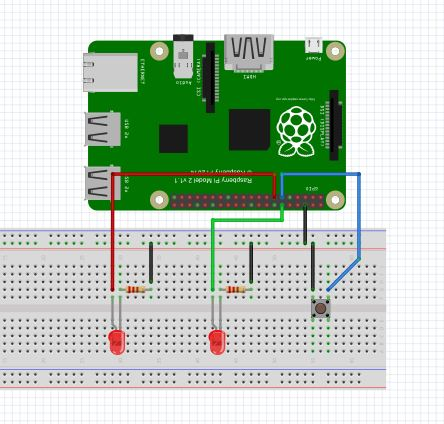
\includegraphics[scale = 0.6]{switch_interrupt}
    \caption{Fritzing Circuit Diagram}
\end{figure}
\subsection*{Assembly of hardware}
\subsection*{Step 1}
Pin 11 is connected to switch and other terminal of switch is grounded.
\subsection*{Step 2}
Pin 12 of Rpi is connected to anode of one of the LED. Cathode of LED is connected to ground through a current limiting resistor.
\subsection*{Step 3}
Pin 13 of Rpi is connected to anode of second LED. Cathode of second LED is connected to ground through a current limiting resistor.

\subsection*{Interrupt on Raspberry Pi using SPI protocol}
\textbf{Description:} \\
SPI is a single-master communication protocol. This means that one
central device initiates all the communications with the slaves. When the SPI master wishes to send data to a slave and/or request information from it, it selects slave by pulling the corresponding SS line low and it activates the clock signal at a clock frequency usable by the master and the slave. The master generates information onto MOSI line while it samples the MISO line.\\
\textbf{Problem Statement:} \\
Connect RPi as SPI master and Arduino as SPI slave and generate an SPI interrupt on RPi.\\
\textbf{Circuit Diagram}  \\
\begin{figure}[H]
    \centering
    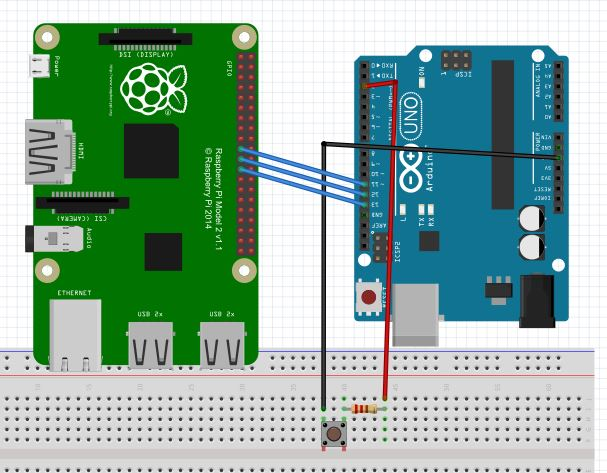
\includegraphics[scale = 0.6]{rpi_with_arduino_spi}
    \caption{SPI Interrupt using RPi as master and Arduino as slave.}
\end{figure}
\subsection*{Assembly of hardware}
\subsection*{Step 1}
Pin 11 of arduino is connected to MOSI(i.e pin 19) of RPi.
\subsection*{Step 2}
Pin 12 of arduino is connected to MISO(i.e pin 21) of RPi.
\subsection*{Step 3}
Pin 12 of arduino is connected to SCLK(i.e pin 23) of RPi.
\subsection*{Step 4}
One terminal of switch is connected to resistor and other terminal to ground.
\subsection*{Step 5}
Other terminal of resistor is connected to digital pin 2 of Arduino.

\subsection*{Interrupt on Raspberry Pi using I2C protocol}
\textbf{Description:} \\
The Inter-integrated Circuit (I2C) Protocol is a protocol intended to allow multiple slave digital integrated circuits (chips) to communicate with one or more master chips. I2C requires a mere two wires, like asynchronous serial, but those two wires can support up to 1008 slave devices. I2C can support a multi-master system, allowing more than one master to communicate with all devices on the bus (although the master devices can't talk to each other over the bus and must take turns using the bus lines). Whenever CPU receives interrupt request from external device using I2C protocol.Control goes to receives data from devices. After that control returns to its main program execution.\\
\textbf{Problem Statement:} \\
Connect RPi as I2C master and Arduino as I2C slave and generate an I2C interrupt on RPi.\\
\newpage
\textbf{Circuit Diagram}  \\
\begin{figure}[H]
    \centering
    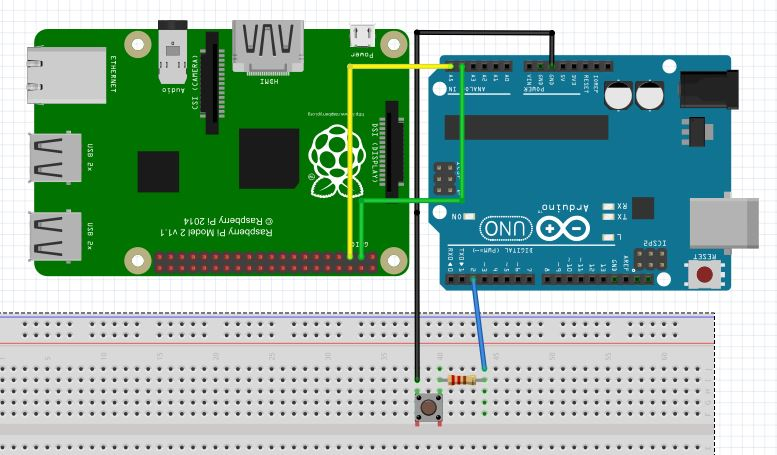
\includegraphics[scale = 0.6]{rpi_with_arduino}
    \caption{I2C Interrupt using RPi as I2C master and Arduino as I2C slave.}
\end{figure}
\subsection*{Assembly of hardware}
\subsection*{Step 1}
Pin 3(SDA) of Rpi is connected to analog pin A4 of Arduino.
\subsection*{Step 2}
Pin 5(SCL) of Rpi is connected to analog pin A5 of Arduino.
\subsection*{Step 3}
One terminal of resistor is connected to switch and other terminal to digital pin 2 of Arduino.
\subsection*{Step 4}
One terminal of switch is connected to resistor and other terminal to ground.
\section{UART Communication between Firebird V and Raspberry Pi}
\textbf{Description:} \\
In Serial Interrupt, whenever CPU receives interrupt request from external device serially(UART), Control goes to receives data from devices. After that control returns to its main program execution.\\
\textbf{Problem Statement:} \\
Connect Raspberry Pi to Firebird V through USB cable and control Firebird V by giving commands in the form of data serially from RPi.
\textbf{Connection Image:} \\
\begin{figure}[H]
    \centering
    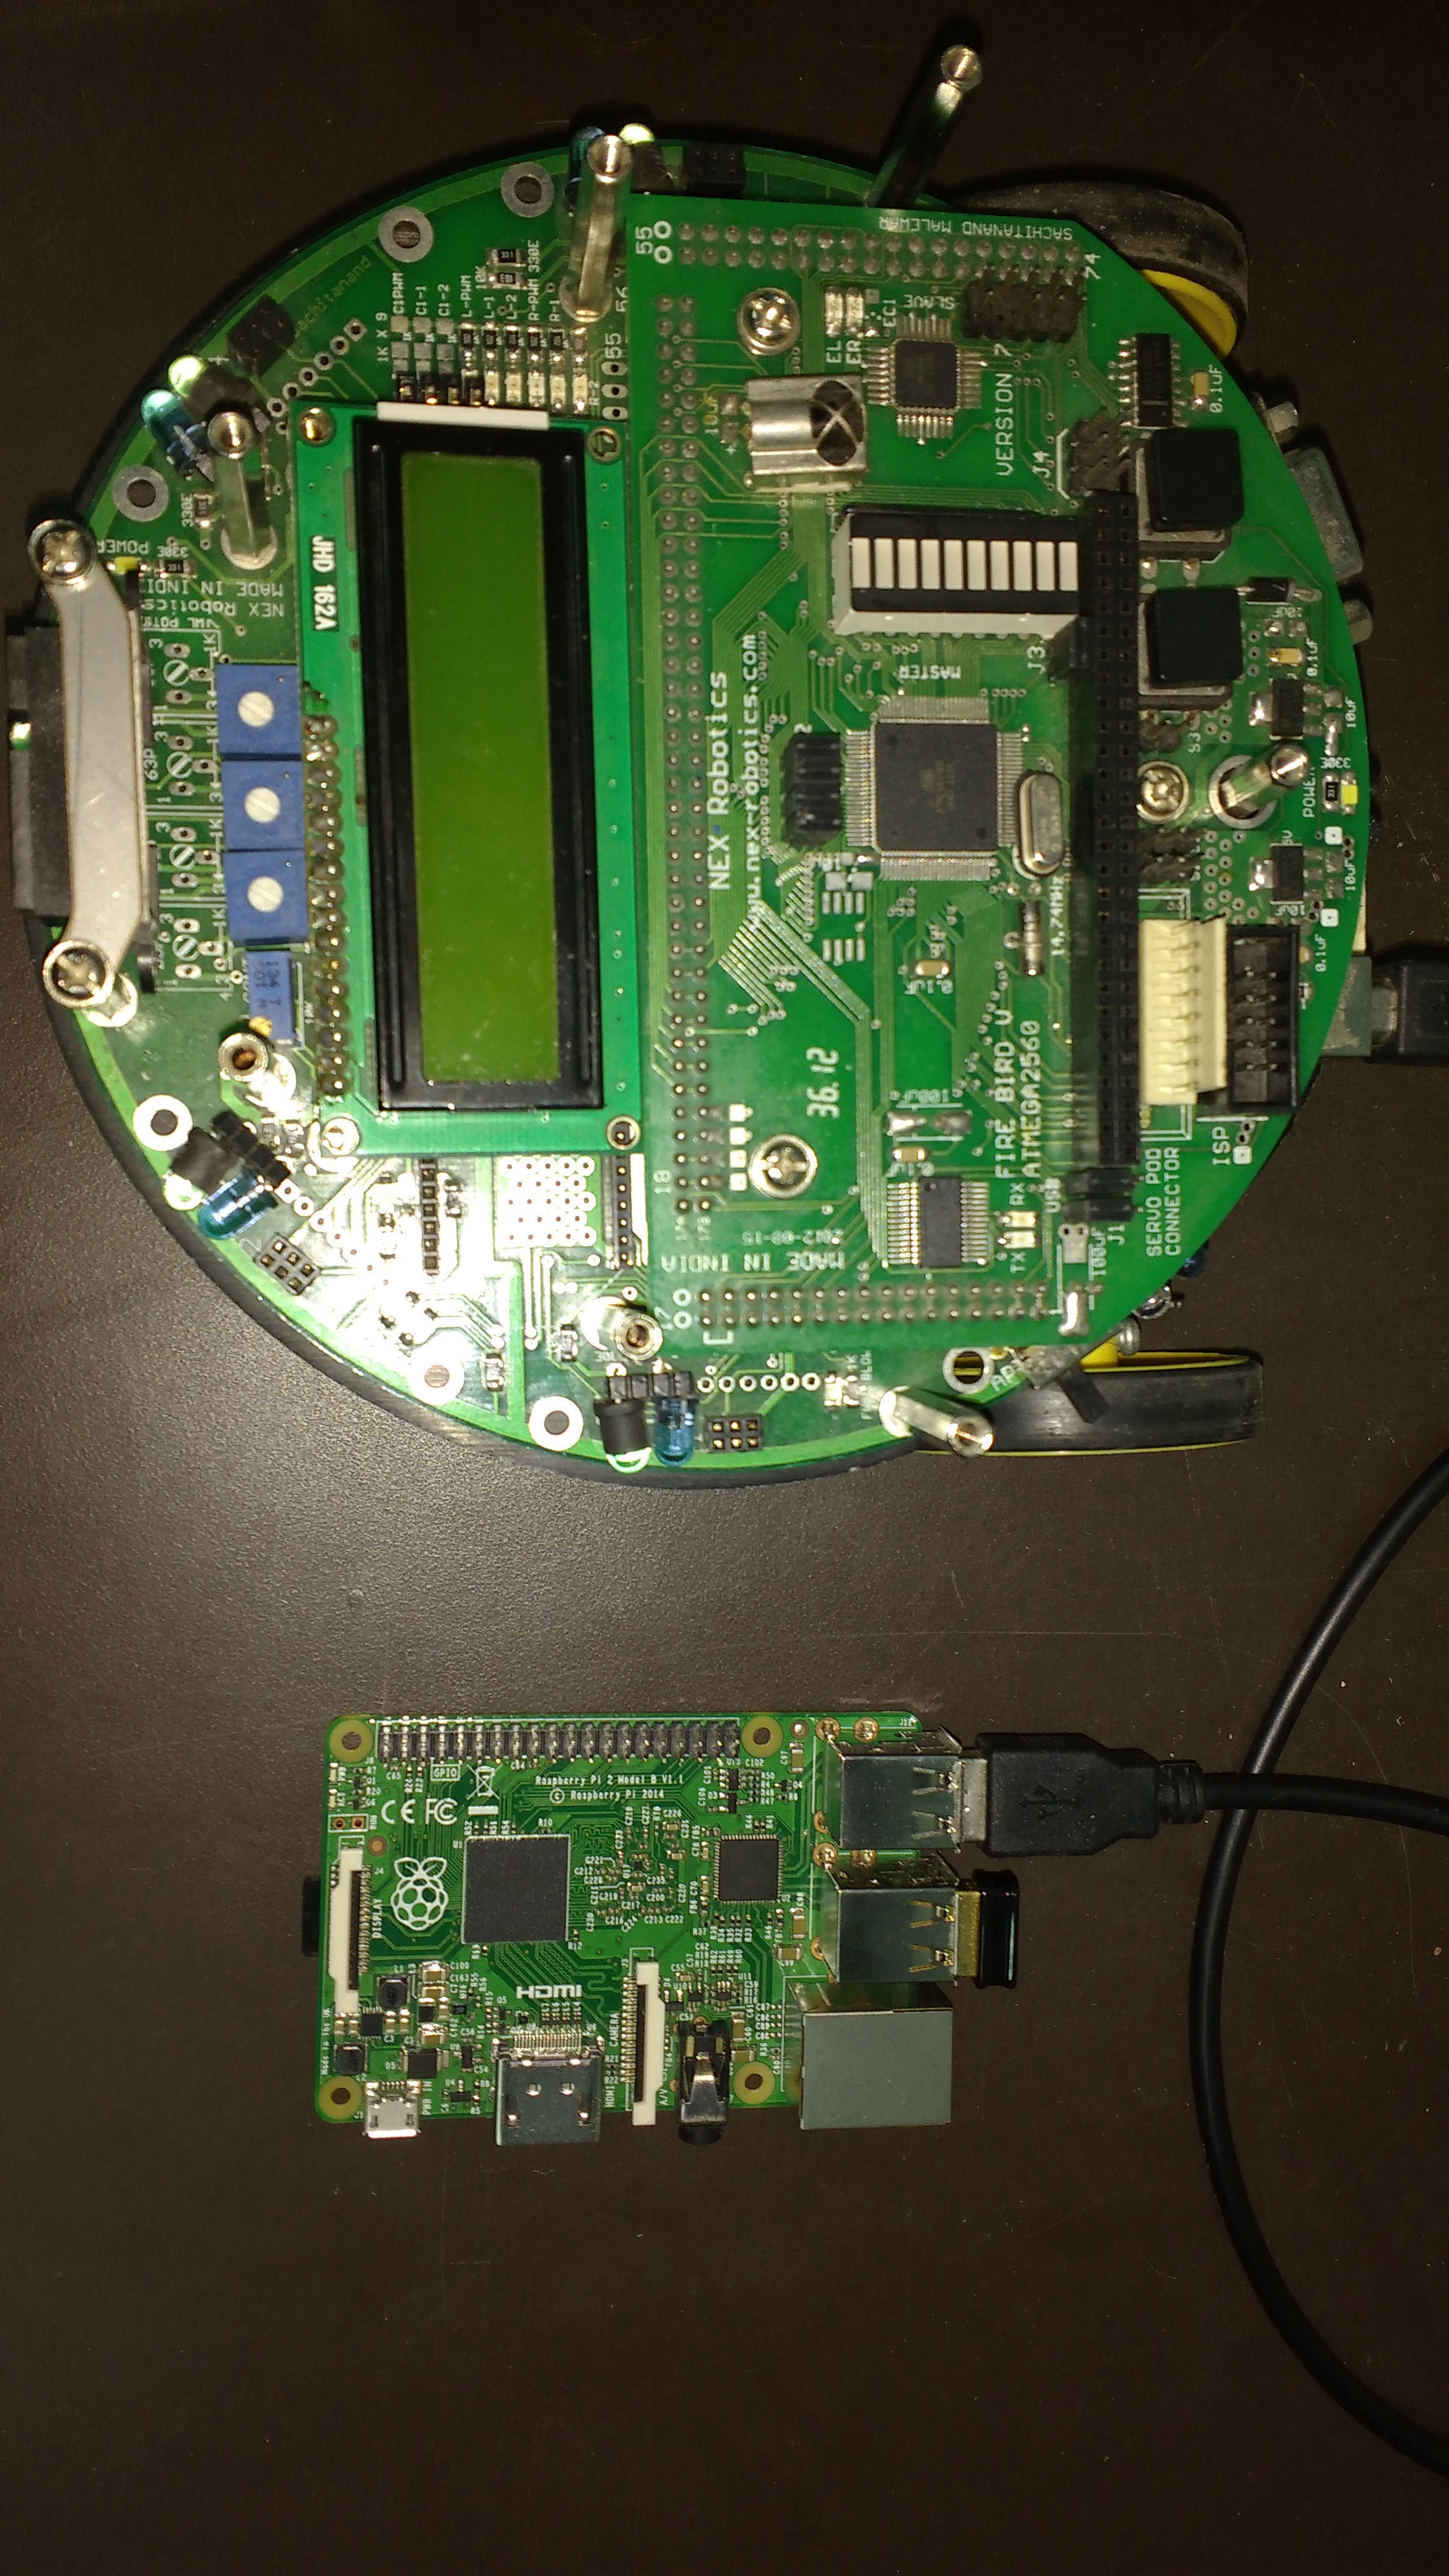
\includegraphics[scale = 0.05]{fff}
    \caption{UART communication between RPi and Firebird V}
\end{figure}

\newpage
\section{Software and Code}
\href{https://github.com/eYSIP-2016/eYSIP-Raspberry_Pi_Development_Board}{Github link} for the repository of code.

\section{Use and Demo}

\href{https://youtu.be/oxJpwd1q_dY}{Youtube Link} of Accessing GPIO pins of RPi. \\
\href{https://youtu.be/Fn3AqdrCMGo}{Youtube Link} of External Interrupt on Raspberry Pi.\\
\href{https://youtu.be/dhToItyDWhE}{Youtube Link} of I2C Enabling on RPi.\\
\href{https://youtu.be/5fbYMdtAb2E}{Youtube Link} of SPI Enabling on RPi.\\
\href{https://youtu.be/bD0IaSN4_MM}{Youtube Link} of Interfacing Port expander MCP23017 to RPi.\\
\href{https://youtu.be/CWC4LPlKH_k}{Youtube Link} of ADC MCP3008. \\
\href{https://youtu.be/3ISq36l3NLc}{Youtube Link} of Bluetooth communication. \\
\href{https://youtu.be/qROTqvKYI3w}{Youtube Link} of PWM driver PCA9685 IC.   \\


\section{Future Work}
Make a PCB Shield for Raspberry Pi which will enhance capability of Firebird V robot.\\
Raspberry Pi is an Excellent tool for Dynamic and Real time Image Processing. So, by using Raspberry Pi instead of AtMega2560 on Firebird V we can implement much complex themes comprising image processing, as the 
programming in python makes it much easier.
\section{Bug report and Challenges}
\begin{itemize}
    \item Communicating Raspberry Pi with ATMega2560 through UART communication protocol causes a lot of delay which can make the programming task much complicated and the program becomes inefficient.
    \begin{enumerate}
        \item Object Tracking of Firebird V Robot using 3 Sharp IR Sensors using UART communication between Raspberry Pi and ATMega2560.
        \item Courier Service theme of eYRC+ using UART communication between Raspberry Pi and ATMega2560.
        \item Obstacle Avoidance Robot using UART communication between Raspberry Pi and ATMega2560.
    \end{enumerate}
     These ideas did not work due to delay in communication because of which line following is not at all effective.
    \item SPI interrupt and I2C interrupt on Raspberry Pi using RPi as Master and Arduino as slave.  
\end{itemize}

\begin{thebibliography}{li}
\bibitem{wavelan97}
Raspbian Jessie OS Installation,
{\em https://www.engadget.com/2012/09/04/raspberry-pi-getting-started-guide-how-to/}
\bibitem{wavelan97}
SPI and I2C communication protocol
{\em www.byteparadigm.com/applications/introduction-to-i2c-and-spi-protocols/}
\bibitem{wavelan97}
I2C configuration
{\em https://learn.adafruit.com/
adafruits-raspberry-pi-lesson-4-gpio-setup/
configuring-i2c}
\bibitem{wavelan97}
Pulse Width Modulation
{\em http://www.electronics-tutorials.ws/blog/
pulse-width-modulation.html}
\bibitem{wavelan97}
Software Interrupt
{\em https://www.techopedia.com/denition/22195/software-interrupt}
\bibitem{wavelan97}
Port expander MCP23017 IC
{\em https://www.mathworks.com/examples/matlab/4547-add-digital-i-o-pins-to-raspberry-pi-hardware-using-mcp23017}
\bibitem{wavelan97}
Queries regarding Raspberry Pi
{\em http://stackoverflow.com/questions/tagged/raspberry-pi}
\bibitem{wavelan97}
Libraries for progrmming different IC's or modules
{\em https://github.com/adafruit}
\end{thebibliography}


\end{document}

